\documentclass[]{article}

\usepackage{pgf-pie}

\title{Natural Language processing for Knowledge Representation} \author{Jens
  Claes}

\begin{document}

\maketitle

\begin{abstract}

\end{abstract}

\section{Probleemstelling}
\paragraph{} Bedrijfsprocessen worden geregeld door specificaties. Deze worden vaak
geschreven in een natuurlijke taal, door een domein expert. Vervolgens worden
deze specificaties vertaald naar uitvoerbare programma's. Bij deze vertaling
slopen er vaak fouten in. Bovendien zijn er vaak meerdere programma's die elk
opnieuw de specificatie moeten implementeren. Zo ontstaan er niet allen
inconsistenties met de specificatie, maar ook tussen de verschillende
programma's onderling zijn er inconsistenties. Ten slotte is het moeilijke om de
specificatie achteraf nog aan te passen omdat alle programma's dan aangepast
moeten worden.

\paragraph{} Het antwoord van de academische wereld op deze problemen, zijn ``Knowledge Base
Systems'' (KBS). In dit paradigma worden de specificaties in natuurlijke taal
vertaald naar specificaties in een formele taal. Deze formele specificatie wordt
gebruikt in alle programma's. Zo is het niet meer mogelijk dat de programma's
onderling inconsistent zijn. Ze gebruiken namelijk allemaal de formele
specificatie. Daardoor is ook het aanpassen van de specificatie makkelijker.
Enkel de formele specificatie moet aangepast worden, de programma's blijven
hetzelfde.

\paragraph{} Het probleem met deze aanpak is dat er nog steeds een vertaling moet gebeuren
van natuurlijke taal naar een formele taal. De specificatie in natuurlijke taal
wordt vaak opgesteld door een domein expert die formele talen niet machtig is.
De formele specificatie wordt dan weer opgesteld door een KBS expert. Deze
persoon kent formele talen maar heeft een beperkte kennis van het domein. Door
deze mismatch van kennis, is de feedback loop tussen de twee experten beperkt.
Het is dus nog steeds mogelijk dat er fouten sluipen in de vertaling.

\paragraph{} De vraag rijst dus of we een formele taal kunnen ontwerpen die toegankelijk is
voor domein experten, rijk genoeg is voor praktische problemen en toepasbaar is
binnen het KBS paradigma.

\paragraph{} Deze thesis onderzoekt of een formele natuurlijke taal het antwoord is op die
vraag. Natuurlijke taal wordt immers al gebruikt bij het opstellen van de
specificatie. Figuur \ref{fig:natural-language-use} toont het gebruik van
natuurlijke taal in vereistenanalyse in 1999. Slechts 5 procent werd toen in een
formele taal opgesteld. 16 procent werd in gestructureerde natuurlijke taal
opgesteld. Dit wil zeggen dat de specificatie in een natuurlijke taal is
opgesteld maar slechts een beperkt aantal zinsconstructies zijn toegestaan, om
de leesbaarheid te verhogen.

\begin{figure}
  \label{fig:natural-language-use}
  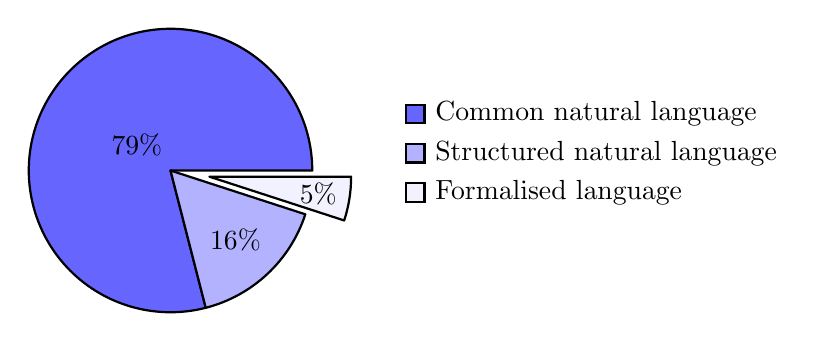
\begin{tikzpicture}
      \pie[text = legend, radius = 1.8, explode = {0, 0, 0.5}, color = {blue!60, blue!30, blue!5}]{79/Common natural language, 16/Structured natural language, 5/Formalised language}
  \end{tikzpicture}
  \caption{Gebruik van natuurlijke taal in vereistenanalyse in 1999 (van figuur 5 in \cite{Luisa2004})}
\end{figure}

\paragraph{} In deze thesis ontwerpen we een nieuwe gestructureerde natuurlijke taal
met als doel dat deze taal leesbaar is voor de domein expert, de KBS expert en
machines. Zo kan een programma de formele specificatie opstellen vanuit de
specificatie in de natuurlijke taal. Er is dan nog maar 1 bron van waaruit alles
geregeld wordt. Inconsistenties zijn niet meer mogelijk. Bovendien kan men nog
steeds makkelijk de specificatie aanpassen.

\section{Literatuurstudie}
\subsection{Circe \cite{Ambriola1997}}
			
\section{Referenties}
\bibliographystyle{plain}
\bibliography{tekst}

\end{document}


% LocalWords: KBS Systems Knowledge programma's
